% !TEX program = xelatex
% !BIB program = biber

\documentclass{VSAnote}

\providecommand\VSAreportpath{../VSAreport}
\usepackage{mdframed}

\usepackage{tikz}

\usepackage{changepage}
\newenvironment{info}{%
	\vspace{\baselineskip}
	\begin{adjustwidth}{20mm}{10mm}%
	\begin{flushleft}
	\itshape\footnotesize%
	\makebox[0pt][r]{\raisebox{-9mm}[1.5ex][0pt]{\includegraphics[width=10mm]{\VSAreportpath/icons/denken}}\hspace{5mm}}\ignorespaces%
	}{%
	\end{flushleft}
	\end{adjustwidth}%
	\vspace{\baselineskip}
	}
\addbibresource{\VSAreportpath/references.bib} 




\begin{document}
	
	
	
	
	
\title{Wat is een statistiek?}
\author{Jorre Vannieuwenhuyze}
\titlepage

\tableofcontents
\clearpage


	% gal-ograjensek-2017-official-statistics-and-statistics-education-bridging-the-gap.pdf
	% 978-3-031-20748-8_3.pdf
	% 978-3-031-20748-8_13.pdf
	% What do citizens need to know about real-world statistical models and the teaching of data modeling, in Reasoning-with-data-models-and-modeling-in-the-big-data-era-Editors-Colophon.pdf
	
	% Porciani, L., & Rondinella, T. (2019). Teaching official statistics in universities. Recommendations from a direct experience. Statistical Journal of the IAOS, 35(3), 425-433.
	% COVID-19 and Numeracy.pdf
	
	% ndifwa-saxena-2020-bridging-the-gap-between-official-statistics-and-theoretical-statistics.pdf
	% boek: https://link.springer.com/book/10.1007/978-3-030-31492-7
	% Allin, P. (2021). Opportunities and challenges for official statistics in a digital society. Contemporary Social Science, 16(2), 156-169.
	% biemer-et-al-2014-a-system-for-managing-the-quality-of-official-statistics.pdf
	
	% Data_Organisation_and_Process_Design_Based_on_Func.pdf
	
	% Aftoetsen welke terminologie wordt gebruikt in de GSIM
	
	
	% 1. Babbie, Earl R. (2020). The Practice of Social Research (15th ed.)
	%Publisher: Cengage Learning
	%Where it’s discussed: Chapter 5 – "Conceptualization and Measurement"
	%Why it’s relevant: Babbie gives one of the clearest and most widely taught distinctions:
	%Conceptual definition: describes what a concept means in abstract or theoretical terms.
	%Operational definition: specifies how the concept will be measured or observed in practice.
	%
	% 2. Bryman, Alan (2016). Social Research Methods (5th ed.)
	%Publisher: Oxford University Press
	%Where it’s discussed: Chapter 3 – "Research Designs", and Chapter 7 – "The Nature of Quantitative Research"
	%Key point: Bryman distinguishes conceptual clarity from measurement clarity, and how bridging them is part of operationalization:
	%“Operationalization involves converting concepts into indicators.”
	%
	% 3. Neuman, W. Lawrence (2014). Social Research Methods: Qualitative and Quantitative Approaches (7th ed.)
	%Publisher: Pearson
	%Where it’s discussed: Chapter 4 – "Conceptualization and Measurement"
	%Notable strength: Offers practical examples (e.g., how to define "poverty" conceptually and then operationally).
	
	
	%Adèr, H.J., Mellenbergh, G.J., & Hand, D.J. (2008).
	%Advising on Research Methods: A Consultant's Companion. Huizen: Johannes van Kessel Publishing.
	%Bevat toelichting over abstracte versus concrete concepten, en over operationalisatie.
	%
	%Baarda, D.B., & De Goede, M.P.M. (2020).
	%Basisboek Methoden en Technieken. Noordhoff.
	%Geeft onderscheid tussen conceptueel en operationeel niveau, en bespreekt enkelvoudige en meervoudige concepten met voorbeelden zoals "welzijn", "tevredenheid", "leeftijd", enz.
	%
	%Babbie, E. (2020).
	%The Practice of Social Research (15e editie). Cengage Learning.
	%Klassieke bron die het onderscheid maakt tussen abstracte concepten, indicatoren en meting. Hierin vind je ook uitgebreide voorbeelden van enkelvoudige en meervoudige begrippen.
	%
	%De Vaus, D. (2001).
	%Research Design in Social Research. SAGE.
	%Bevat heldere uitleg over het ontleden van complexe concepten (zoals sociaal kapitaal, armoede, enz.) in meerdere dimensies.
	%
	%OECD en United Nations Statistical Division documenten
	%In internationale richtlijnen over statistische indicatoren (zoals in de OECD Handbook on Constructing Composite Indicators) vind je veel voorbeelden van meervoudige concepten (bv. welzijn, levenskwaliteit) en hun operationalisering in indicatoren.
	
	
	
	
	
	
	
	
	
	
	
	
Voor we bespreken hoe een Nationale Statistische Instantie (NSI) zoals Statistiek Vlaanderen statistieken produceert, moeten we afspreken wat we precies verstaan onder een statistiek. Wat beschouwen we als een statistiek en wat niet? Welke informatie is essentieel om statistieken te produceren en te publiceren? Hoe bepalen we de kwaliteit van statistieken? Het antwoord op al deze vragen komt aan bod in dit hoofdstuk. 
	



	
	
\section{Statistiek als een cijfer}
	
Als je mensen vraagt wat ze verstaan onder een statistiek, zullen velen dit op de eerste plaats definiëren als een cijfer. Die definitie is echter niet volledig. Neem bijvoorbeeld het cijfer ``525\,935'', een statistiek die we publiceren vanuit Statistiek Vlaanderen. Op zichzelf zegt dit cijfer uiteraard zeer weinig. Waarvan zijn er 525\,935? Wat stelt dit getal voor? Waarom publiceren we dat getal? Hoe werd het getal gemeten? Hoe kwalitatief is deze meting? Wie is verantwoordelijk voor dit cijfer? Statistiek gaat dus niet alleen over het berekenen van cijfers, het gaat ook over het beheer van allerhande informatie die bij het cijfer hoort. Deze informatie noemen we \emph{attributen} van het cijfer. Een \emph{statistiek} bestaat dus altijd uit twee onlosmakelijke elementen: het cijfer zelf (ook wel \emph{data} genoemd), én de attributen van dat cijfer (ook wel \emph{metadata} genoemd). Beiden zijn even belangrijk en vormen één geheel \parencite{Wild2018What}. In deze paragraaf gaan we dieper in op verschillende belangrijke attributen van een statistiek. 

\begin{info}
	Merk op dat statistieken niet altijd cijfers zijn, het kunnen ook kwalitatieve observaties zijn of zelfs complexere ``informatie-objecten''. Zo publiceert het Agentschap Binnenlands Bestuur bijvoorbeeld per gemeente een statistiek over de top 10 andere gemeenten waarnaar kinderen heen pendelen voor school. Voor de stad Antwerpen kan de observatie op deze statistiek bijvoorbeeld de volgende tekstuele vector zijn: 
	\begin{quote}
		``\lbrack Antwerpen, Brasschaat, Lier, Brussel, Beveren, Mechelen, \ldots\rbrack''.
	\end{quote}
	Voor de eenvoud verwijzen we in deze tekst echter enkel naar statistieken als eenvoudige cijfers. Cijfers zijn immers veruit de meest voorkomende vorm van statistieken. 
\end{info}	
	
	


	
\subsection{Gebruikersbehoeften}
	
Als een NSI een statistiek publiceert, is dat steeds als antwoord op specifieke \emph{gebruikersbehoeften}. Die gebruikersbehoeften zijn het eerste belangrijke attribuut van de statistiek. 

Het cijfer 525\,935 betekent bijvoorbeeld ``het aantal inwoners van de gemeente Antwerpen in 2019''. Als we dit cijfer vanuit Statistiek Vlaanderen publiceren, betekent dit dat sommige beleidsmakers, onderzoekers of burgers daadwerkelijk graag willen weten hoeveel inwoners Antwerpen telde in 2019. Een Vlaams decreet kan bijvoorbeeld verwijzen naar het aantal inwoners in de Vlaamse gemeenten en verplicht ons dit aantal te publiceren zodat de Vlaamse regering hierop beleid kan uitstippelen. Antwerpse beleidsmakers weten daarnaast waarschijnlijk ook graag hoeveel inwoners hun gemeente telt zodat ze hun diensten hierop kunnen afstemmen. Wetenschappelijke onderzoekers gebruiken de Antwerpse bevolkingsgrootte in 2019, samen met gegevens uit andere jaren en gemeenten, dan weer om bevolkingsgroei en ‐spreiding in Vlaanderen te onderzoeken. Burgers willen misschien wel graag weten hoeveel inwoners Antwerpen telt om te beoordelen of bepaalde Vlaamse subsidies aan de stad gerechtvaardigd zijn of niet.

Verschillende onderdelen van gebruikersbehoeften worden opgelijst in de ``Praktijkcode voor Europese statistieken'' \parencite[zie][]{Eurostat2017European}. Deze praktijkcode schept een kwaliteitskader voor het Europees statistisch systeem (ESS) en legt 16 beginselen vast voor de ontwikkeling, productie en verspreiding van Europese statistieken. Volgens de praktijkcode hebben gebruikers op de eerste plaats behoeften aan \emph{relevante} statistieken. Dit betekent dat de statistiek beantwoordt aan de behoeften van een gebruiker. Daarnaast verwachten gebruikers ook \emph{nauwkeurige} statistieken. Dit betekent dat de statistiek meet wat ze moet meten. Relevantie en nauwkeurigheid zijn sterk aan elkaar gerelateerd, je kan geen relevante statistieken opleveren als ze niet nauwkeurig zijn, maar ze bevatten toch een nuanceverschil die verder in de tekst zal worden uitgelegd. 

Naast relevantie en nauwkeurigheid, somt de praktijkcode ook andere mogelijke verwachtingen op van gebruikers. Gebruikers kunnen bijvoorbeeld ook verwachten dat statistieken \emph{tijdig} en \emph{punctualiteit} zijn. Dit betekent dat de statistieken snel en op duidelijke tijdstippen worden gepubliceerd. Dit laat beleidsmakers immers toe snelle beleidsbeslissingen te nemen in tijden van crisis of wanneer bepaalde beleidsbeslissingen gebonden zijn aan duidelijke juridische deadlines. Gebruikers kunnen ook verwachten dat de statistieken \emph{vergelijkbaar} zijn. Dit betekent dat de gebruiker de statistieken kan vergelijken met eerder verschenen cijfers of met cijfers uit andere landen of regio's. Gebruikers verwachten doorgaans ook dat de statistieken \emph{toegankelijk} zijn. Dit betekent dat gebruikers de statistieken op een gebruiksvriendelijke manier kunnen raadplegen en dat de statistieken gemakkelijk te interpreteren zijn. Als laatste moeten statistieken ook steeds \emph{wettelijk verantwoord} zijn. Dit betekent dat de statistieken worden gepubliceerd conform de wet en regelgeving.

\begin{info}
	Dat cijfers wettelijk verantwoord moeten zijn staat niet expliciet vermeld in de Europese praktijkcode als beginsel. Dit is een duidelijk hiaat in de praktijkcode. Deze vereiste wordt wel impliciet vermeld via beginselen over een institutioneel kader rond statistische geheimhouding en gegevensbescherming. 
\end{info}

\begin{info}
	De verschillende onderdelen van gebruikersbehoeften staan in de praktijkcode opgesomd als beginselen rond statistische output. Daarnaast bevat de ``Praktijkcode voor Europese statistieken'' nog tien andere beginselen rond het institutioneel kader waarbinnen een Nationaal Statistische Instantie (NSI) functioneert en de statistische processen die een NSI installeert. Deze ``beginselen'' kan je echter bekijken als hulpmiddelen om de beginselen rond statistische output waar te maken. 
	
	Zo vereist beginsel 1 dat NSI's professioneel onafhankelijk opereren. Dit betekent dat er geen politieke of andere externe invloeden zijn op het werk van de NSI. Beginsel 6 is hier nauw mee verbonden en vraagt dat NSI's onpartijdig en objectief zijn. Deze beginselen zorgen er dus voor dat de NSI's alle gebruikersbehoeften maatschappijbreed in kaart brengen, hun statistiekproductie hierop afstemmen en daardoor relevante en nauwkeurige statistieken opleveren. Relevante en nauwkeurige statistieken zijn dus de beginselen, onafhankelijkheid en onpartijdigheid zijn enkel hulpmiddelen om deze beginselen waar te maken. 
	
	Beginsel 2 bepaalt dat een NSI een wettelijk mandaat krijgt voor de verzameling van en toegang tot gegevens. Beginsel 3 stelt op haar beurt dat NSI's over voldoende personele, financiële en technische middelen moeten beschikken. Deze beginselen garanderen dat gebruikersbehoeften optimaal in kaart worden gebracht door de NSI en dat aan deze behoeften voldaan wordt met relevante en nauwkeurige statistieken.
	
	Beginsel 4 vraagt om een sterk kwaliteitsbewustzijn bij NSI's. Dit beginsel hangt nauw samen met beginsels 7 en 8, die vereisen dat NSI's deugdelijke methoden en geschikte statistische procedures gebruiken om kwaliteit voortdurend te optimaliseren. Deze beginselen zeggen niet meer en niet minder dan dat NSI's moeten streven naar maximale nauwkeurigheid in hun statistieken en zijn dus volledig redundant.  
\end{info}




	
	
	
\subsection{Conceptuele definitie}

Om gebruikersbehoeften te vervullen, moet een NSI zoals Statistiek Vlaanderen cijfers publiceren met een bepaalde betekenis. Die betekenis noemen we de \emph{conceptuele definitie} van de statistiek \parencite{neuman2014Social, refs toevoegen}. In ons voorbeeld is ``het aantal inwoners van de gemeente Antwerpen in 2019'' dus de conceptuele definitie van de statistiek ``525\,935''. 
	
Een conceptuele definitie bevat doorgaans verschillende delen of componenten. Bij de statistiek over het aantal inwoners in Antwerpen in 2019 kunnen we bijvoorbeeld drie componenten onderscheiden. Ten eerste kijken we naar een gemeente, ten tweede kijken we naar een bepaald jaar, en ten derde kijken we naar een grootheid die we willen meten. Deze componenten noemen we \emph{concepten} \parencite{clark2021Social}. Een concept is dus niet meer dan een idee of betekenis die helpt om statistische gegevens te begrijpen en te ordenen \parencite{GSIM2024}. Het is als een label dat zegt ``Dit is wat we meten''. 

Een concept op zich is echter steeds slechts een containerbegrip. In de praktijk neemt een concept steeds een bepaalde \emph{waarde} aan om de betekenis van een statistiek te verduidelijken. In het voorbeeld is de waarde van het concept gemeente `Antwerpen', de waarde van het concept jaartal `2019', en de waarde van het concept grootheid `het aantal inwoners'. De waarden geven dus betekenis aan het cijfer, niet het concept zelf. 
	
Let op, de afbakening van concepten en waarden in een conceptuele definitie is niet altijd duidelijk en is voor een stukje arbitrair. Zo kan je bijvoorbeeld cijfers publiceren over het aantal inwoners in Antwerpen per bevolkingsgroep (mannen, vrouwen, 0- tot 18-jarigen, 19- tot 64- jarigen, 65+'ers, mensen met Belgische nationaliteit, mensen met buitenlandse nationaliteit, \ldots). Spreken we in deze definitie van één concept ``bevolkingsgroep'' of hebben we hier te maken met meerdere concepten zoals ``geslacht'', ``leeftijd'' en ``nationaliteit''? Concepten kan je ook arbitrair opsplitsen en samenvoegen. Hebben we in het voorbeeld hierboven slechts één concept ``grootheid'' met waarde ``aantal inwoners'', of kan je hier niet beter twee concepten aparte concepten onderscheiden, namelijk het concept ``statistische parameter'' met waarde ``aantal'' en het concept ``eenheid'' met waarde ``inwoners''? Op deze vragen is er geen éénduidig juist of fout antwoord maar we zullen wel een keuze moeten maken om het productieproces voor deze statistieken in de praktijk te organiseren. Dit wordt verder uitgelegd in hoofdstuk \ref{ch:statistiekenbepalen}.
	
	
	
	
\subsection{Operationele definitie}
	
De conceptuele definitie is meestal vaag over wat een cijfer precies weergeeft. In de zin ``het aantal inwoners in Antwerpen neemt toe'' is bijvoorbeeld ``het aantal inwoners'' enkel een abstract idee. Deze woorden vertellen immers niet wie je nu precies meetelt en wie niet om dit aantal te bepalen. De conceptuele definitie van een cijfer vertelt dus weinig over hoe het cijfer precies werd berekend en exact geïnterpreteerd kan worden. Naast de conceptuele definitie heeft elke statistiek daarom ook een \emph{operationele definitie}. Die operationele definitie beschrijft tot in detail hoe het cijfer exact is gemeten en geeft zo de precieze betekenis ervan weer. De operationele definitie is daarom veel uitgebreider dan de conceptuele definitie. De vertaling van de conceptuele definitie naar de operationele definitie noemen we \emph{operationaliseren}.

De operationalisering van een conceptuele definitie betekent in de praktijk dat elk concept vertaald wordt van een abstract idee naar een concrete richtlijn om de conceptwaarden te meten. Concepten variëren echter in hoe concreet of abstract ze zijn \parencite{referentie toevoegen}. Een \emph{concreet concept} verwijst naar een fenomeen dat direct observeerbaar of eenvoudig meetbaar is zonder complexe interpretatie of afleiding. Een voorbeeld van een concreet concept is het aantal huishoudens in een gemeente. Dit is een concreet concept want je kan het rechtstreeks vaststellen op basis van administratieve gegevens (bv. bevolkingsregister). Er is bovendien weinig discussie over wat een huishouden is, zeker als er een duidelijke juridische of administratieve definitie wordt gehanteerd. 
		
Een \emph{abstract concept} verwijst daarentegen naar een idee of fenomeen dat niet rechtstreeks waarneembaar is. Het heeft een zekere mate van theoretische of interpretatieve lading en moet daarom eerst geoperationaliseerd worden naar concretere concepten en conceptwaarden. Een voorbeeld van een abstract concept is sociaal isolement. Sociaal isolement verwijst immers naar een toestand waarin iemand weinig of geen sociale contacten heeft of zich sociaal buitengesloten voelt. Dit kan je niet rechtstreeks meten maar moet je operationaliseren. Dat kan bijvoorbeeld via een lange vragenlijst over, onder andere, het aantal sociale contacten, subjectieve gevoelens van eenzaamheid en deelname aan sociale activiteiten.
	
In de praktijk zijn concepten niet of concreet of abstract, maar kan je ze op een continue schaal plaatsen op het vlak van abstractheid en concreetheid. Het éne concept is al abstracter en moeilijker meetbaar en operationaliseerbaar terwijl een ander concept redelijk concreet is en vrij direct geoperationaliseerd en geobserveerd kan worden.  
	
Neem opnieuw het cijfer 525\,935 als voorbeeld om het aantal inwoners van Antwerpen in 2019 weer te geven. De volledige operationele definitie van dit cijfer luidt:
\begin{quote} 
	\makebox[0pt][r]{``}%
	De grootte van de wettelijke bevolking op 1 januari 2019, 0.00 uur, van de gemeente Antwerpen (NIS 11002 in 2019). De grootte van de wettelijke bevolking wordt gedefinieerd en aangeleverd door Statbel op basis van het Rijksregister van de natuurlijke personen. Dit Rijksregister bevat, onder andere, het bevolkingsregister en het vreemdelingenregister die de wettelijke bevolking bepalen. Het bevolkingsregister bevat alle Belgen en buitenlanders die gemachtigd zijn tot vestiging op het Belgisch grondgebied, en het vreemdelingenregister bevat alle buitenlanders die toegelaten of gemachtigd zijn tot een verblijf van meer dan 3 maanden op het Belgisch grondgebied, hetzij voor bepaalde of onbepaalde duur. 
	
	Bepaalde categorieën buitenlanders (vb. diplomatiek en consulair personeel) zijn vrijgesteld van inschrijving in de bevolkingsregisters en worden daardoor niet meegerekend bij de wettelijke bevolking. In sommige gevallen kunnen zij op eigen vraag wel ingeschreven worden. Enkel in dat geval worden zij meegerekend in de bevolkingscijfers.
		
	Het Rijksregister omvat verder ook een wachtregister voor asielzoekers en een wachtregister voor EU‐burgers. Het wachtregister voor asielzoekers bevat alle verzoekers om internationale bescherming die worden ingeschreven door de Dienst Vreemdelingenzaken (DVZ). In 1995 besliste Statbel de personen in dit wachtregister niet meer mee te tellen bij de wettelijke bevolking. Pas nadat asielzoekers worden overgeschreven van het wachtregister naar het bevolkingsregister of het vreemdelingenregister, worden zij opgenomen in de bevolkingsstatistieken van Statbel. Zo'n overschrijving naar het bevolkingsregister of het vreemdelingenregister gebeurt na erkenning als vluchteling, na toekenning van een statuut subsidiaire bescherming, of na verwerving van een verblijfsvergunning om een andere reden.
		
	Verder bevat het Rijksregister ook een wachtregister voor EU‐burgers in afwachting van woonstcontrole. Deze personen worden evenmin meegeteld bij de wettelijke bevolking. Pas na woonstcontrole worden deze personen overgeschreven naar het vreemdelingenregister en worden zij meegeteld in de wettelijke bevolking.%
	''
\end{quote}

Deze operationele definitie bevat een duidelijke operationalisering van elk concept afzonderlijk (zie Tabel \ref{tab:operationaliseren}). Het concept ``gemeente'' wordt geoperationaliseerd als de gemeente volgens de NIS-code indeling in 2019. Het concept ``jaar'' wordt geoperationaliseerd als de toestand op 1 januari, 0.00 uur, van een kalenderjaar. Het concept ``grootheid'' wordt geoperationaliseerd als het aantal personen in de wettelijke bevolking met bijhorende precieze definitie van wie meegerekend wordt in de wettelijke bevolking en wie niet. Het voorbeeld toont ook dat de concepten in een conceptuele definitie doorgaans abstract zijn. Zelfs een eenvoudige concept zoals ``grootheid'' met waarde ``aantal inwoners'' bevat al een zekere abstractie. De ``grootte van de wettelijk bevolking'' is duidelijk een concretere conceptwaarde en kan worden gebruikt om de abstractere conceptwaarde ``aantal inwoners'' te meten.

\begin{table}
\caption[Van conceptuele naar operationele definitie]{Operationaliseren betekent dat alle abstracte concepten in de conceptuele definitie worden vertaald naar concrete en observeerbare concepten in de operationele definitie}
\label{tab:operationaliseren}
\begin{tblr}{
	colspec={lX[l]X[l]X[l]},
	column{1} = {bg=softsteelblue,fg=white,colsep=2pt},
	row{1} = {bg=deepslateblue,fg=white},
	hline{Z} = {deepslateblue},
	vline{1,Z} = {deepslateblue}
	}
& Concept 1 & Concept 2 & Concept 3 \\ 
\begin{tabular}[c]{@{}l@{}}conceptuele\\definitie\end{tabular} &  aantal inwoners & in Antwerpen & in 2019 \\
& \qquad$\downarrow$ & \qquad$\downarrow$ & \qquad$\downarrow$ \\  
\begin{tabular}[t]{@{}l@{}}operationele\\definitie\end{tabular}  &  aantal inwoners volgens de wettelijke bevolking & 
in Antwerpen volgens NIS-code 11002 in 2019 &
op 1 januari 2019, 0.00 uur\\
\end{tblr}
\end{table}

De operationele definitie van het aantal inwoners in Antwerpen in 2019 illustreert dat zelfs relatief eenvoudige statistieken al een tamelijk lange operationele definitie vereisen. De lengte van een operationele definitie kan dan ook sterk variëren. Voor een eenvoudig cijfer afgeleid uit officiële registers, zoals het aantal inwoners in Vlaamse gemeenten, kunnen enkele korte paragrafen volstaan. Bij complexere statistieken, zoals bijvoorbeeld de gemiddelde opinie van inwoners gemeten via een bevraging, is daarentegen een uitgebreid rapport nodig met alle details over, onder andere, het enquêtedesign, de steekproeftrekking, het ontwerp van de vragenlijst, de opvolging van respondenten, statistische correcties voor meet- en selectiefouten en de statistische analysemethoden.

de operationele definitie van het aantal inwoners in Antwerpen in 2019 illustreert ook dat tijdens de vertaalslag van conceptuele naar operationele definitie keuzes moeten worden gemaakt. Die keuzes kunnen ervoor zorgen dat andere cijfers worden bekomen. Het cijfer 525\,935 verwijst bijvoorbeeld naar het jaar 2019, maar wordt wel enkel gemeten op 1 januari 2019. Een vergelijkbaar maar ander cijfer kon worden berekend als ``jaar'' op een andere wijze werd geoperationaliseerd, bijvoorbeeld door een andere dag in het jaar te kiezen in plaats van 1 januari of door het jaargemiddelde te berekenen over alle dagen. Bovendien verwijst 525\,935 naar de wettelijke bevolking gerapporteerd door Statbel en in die wettelijke bevolking worden personen uit de wachtregisters niet meegeteld. Eurostat, daarentegen, rapporteert niet de wettelijke bevolking maar de verblijvende bevolking inclusief personen in het wachtregister en publiceert daarom andere cijfers dan Stabel en Statistiek Vlaanderen, ook al interpreteren de meeste gebruikers zowel de Europese als de Belgische en Vlaamse cijfers gewoon als de ``bevolkingsgrootte''. Verder verwijst het cijfer 525\,935 naar de gemeente Antwerpen zoals gedefinieerd door NIS‐code 11002 in 2019. Door fusies, splitsingen of grensaanpassingen verandert het grondgebied van sommige gemeenten over de tijd; bijvoorbeeld, in 2025 fuseerde Antwerpen met Borsbeek, waardoor het grondgebied veranderde. We zouden opnieuw een vergelijkbaar maar ander cijfer kunnen berekenen voor alle personen in 2019 die op dat moment woonden in wat we nu als de gemeente Antwerpen beschouwen, inclusief Borsbeek dus. 

Een operationele definitie heeft dus twee doelen. Het eerste doel is om duidelijkheid te scheppen over de gemaakte keuzes om een statistiek te berekenen. Hierdoor kan iedereen de cijfers reproduceren en creëer je transparantie. Als twee onderzoekers met dezelfde operationele definitie verschillende cijfers bekomen, is de definitie onvolledig of onnauwkeurig omdat bepaalde concepten nog te abstract zijn. 

\begin{info} 
	In theorie leidt een operationele definitie steeds tot één exact resultaat. In de praktijk is dit echter niet steeds het geval. Als het productieproces bijvoorbeeld een willekeurige steekproef of simulatie bevat, kan het cijfer variëren. Toch blijft de operationele definitie als idee ook in zo'n situaties overeind. Twee onderzoekers zouden in zo'n situatie op basis van dezelfde operationele definitie gemiddeld steeds tot hetzelfde cijfer moeten komen wanneer zij hun productieproces blijven herhalen. Het gebied van de inferentiële statistiek biedt hiervoor het theoretisch kader, maar dat gaat voorbij het doel van deze handleiding.
\end{info}
	
Het tweede doel van de operationele definitie is duidelijkheid te scheppen over de vergelijkbaarheid van cijfers. Je kan bijvoorbeeld niet zomaar de grootte van de wettelijke Antwerpse bevolking in 2019 vergelijken met de grootte van de verblijvende Antwerpse bevolking in 2020. Dit zou immers kunnen leiden tot onjuiste conclusies over bevolkingsgroei of -krimp, ook al worden beide cijfers conceptueel geïnterpreteerd als de Antwerpse ``bevolkingsgrootte''.
	
Je zou je nu kunnen afvragen waarom we eigenlijk conceptuele definities opstellen als ze, in tegenstelling tot de operationele definitie, niet concreet en voldoende accuraat zijn? Toch zijn er goede redenen om voor elke statistiek een goede conceptuele definitie te bepalen. Ten eerste is de conceptuele definitie een pak handiger in gebruik dan de operationele definitie om cijfers te rapporteren. Statistiekgebruikers beperken zich doorgaans tot de conceptuele definitie om cijfers te benoemen en te interpreteren, ook al zijn er binnen dezelfde conceptuele definitie meerdere operationele definities mogelijk. Iemand die praat over het aantal inwoners in Antwerpen in 2019 zal dit eenvoudigweg de ``Antwerpse bevolkingsgrootte'' noemen en niet de hele operationele definitie afratelen. Ten tweede hebben de nuances in de operationele definitie vaak weinig invloed op beleidskeuzes of onderzoeksconclusies die gebruikers maken op basis van de cijfers. Of je nu de feitelijke of de verblijvende bevolking gebruikt om de bevolkingsomvang in Antwerpen te meten, en of je dit nu doet aan het begin of in het midden van het kalenderjaar, de meeste gebruikers zullen min of meer dezelfde conclusies trekken over bevolkingsgroei als ze deze cijfers over de jaren heen vergelijken.
	
	

	
	
	
	
	
	
	
\subsection{Kwaliteit}
	
We zagen reeds dat een statistiek wordt beschreven door drie attributen. Ze ontstaat vanuit gebruikersbehoeften en deze behoeften vertalen we naar een conceptuele definitie en vervolgens een operationele definitie (zie Figuur \ref{fig:beschrijvingstatistiek}). In een ideale situatie zijn de conceptuele en operationele definitie afgestemd op de gebruikersbehoeften. Wanneer dat niet het geval is, heeft de statistiek een \emph{kwaliteitsprobleem}. Dit kan zich voordoen bij alle soorten gebruikerscriteria binnen de gebruikersbehoeften.
	
\begin{figure}
\caption[De drie beschrijvende elementen van een statistiek.]{De kwaliteit van een statistiek wordt gedefinieerd door de verhouding tussen drie elementen.}
\label{fig:beschrijvingstatistiek}
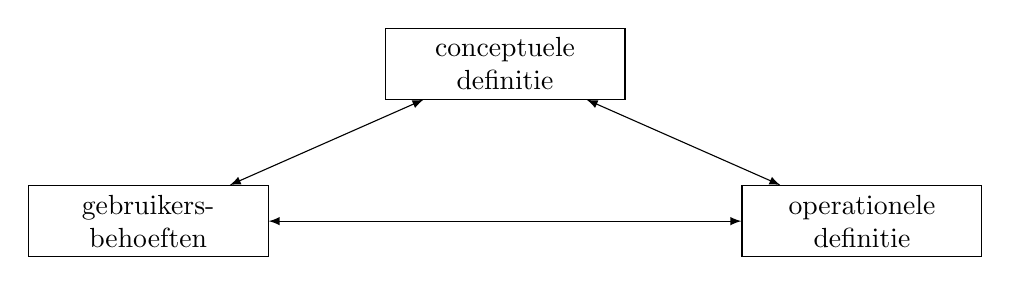
\begin{tikzpicture}[
	x=\linewidth,
	y=2cm,
	box/.style={draw,text width=8em,align=center},
	arr/.style={latex-latex}
	]
	\node[box,anchor=west] (N1) at (0,0) {gebruikers-\\behoeften};
	\node[box,anchor=center] (N2) at (0.5,1) {conceptuele\\definitie};
	\node[box,anchor=east] (N3) at (1,0) {operationele\\definitie};
	\draw[arr] (N1) to (N2);
	\draw[arr] (N2) to (N3);
	\draw[arr] (N1) to (N3);
\end{tikzpicture}
\end{figure}

\paragraph{Relevantie}

Er is een probleem op het vlak van \emph{relevantie} als de conceptueel gedefinieerde statistieken van een NSI niet in overeenstemming zijn met de gebruikersbehoeften. Dit probleem kan optreden in twee richtingen. Op de eerste plaats kan er behoefte zijn aan bepaalde statistieken maar produceert de NSI ze niet. Op de tweede plaats kan de NSI echter ook statistieken produceren waar helemaal geen behoefte aan is. Ook in die situatie kan de kwaliteit van de statistiekproductie verbeterd worden. De NSI verliest dan immers tijd en energie aan irrelevante statistieken terwijl ze die tijd en energie ook kan inzetten op een andere manier. In beide situaties vervult de NSI haar rol als publieke en onafhankelijke statistiekdienst onvoldoende.

Een relevantieprobleem kan ook ontstaan als er een wanverhouding ontstaat tussen gebruikersbehoeften en de operationele definitie van een statistiek. In ons Antwerps voorbeeld kunnen gebruikers bijvoorbeeld het cijfer 525\,935 systematisch interpreteren als de grootte van de verblijvende Antwerpse bevolking in plaats van de wettelijke bevolking omdat ze gewoonweg beleidsmatig voornamelijk de grootte van de verblijvende bevolking nodig hebben. In dit soort situaties moeten we onderzoeken of de operationele definitie aangepast kan worden aan de behoeften. In ons hypothetisch voorbeeld is het misschien aangeraden dat we voortaan Eurostat volgen en de grootte van de verblijvende bevolking publiceren in plaats van de wettelijke bevolking.  

In vele situaties is een evaluatie van de operationele definitie in functie van gebruikersbehoeften echter geen zwart-wit-verhaal. Er kunnen zich immers situaties voordoen waarin de gebruikte operationele definitie voldoet voor de ene gebruiker maar niet voor een andere gebruiker. Zo kan de statistiek over bevolkingsgrootte op basis van de wettelijke bevolking voldoende zijn voor heel wat gebruikers, behalve voor een specifieke beleidsmaker die het woonbeleid in Antwerpen moet bepalen. Deze beleidsmaker heeft misschien nood aan exacte cijfers over de verblijvende bevolking in plaats van de wettelijke bevolking. Ook in zo’n geval is er een gebruikersbehoefte waar we met de statistiek ``Aantal inwoners in Antwerpen'' niet aan voldoet, ook al voldoet deze statistiek wel voor de behoeften van de meeste andere gebruikers.

In situaties met verschillende niet-overlappende gebruikersbehoeften kan een NSI zoals Statistiek Vlaanderen besluiten niet langer één statistiek te publiceren maar verschillende statistieken. Zo kunnen we besluiten niet één statistiek te publiceren over ``het aantal inwoners in Antwerpen'', maar wel twee afzonderlijke statistieken: ``de wettelijke bevolkingsgrootte van Antwerpen`` en ``de verblijvende bevolkingsgrootte van Antwerpen''. Zo wordt voldaan aan de specifieke noden van alle gebruikers. Merk op dat in zo'n situaties zowel de conceptuele definities als de bijhorende operationele definities verder verfijnd en aangepast moeten worden. Uiteraard moeten dit soort keuzes steeds gebeuren vanuit praktische en pragmatische overwegingen in functie van de middelen en het personeel die we ter beschikking hebben. We kunnen in bovenstaande situatie bijvoorbeeld ook besluiten om niet te voldoen aan de noden van deze éne specifieke beleidsmaker omdat dit te veel energie zou vragen voor wat het oplevert.

	
\paragraph{Nauwkeurigheid}

Er is een probleem op het vlak van \emph{nauwkeurigheid} als een statistiek niet meet wat ze moet meten of, anders verwoord, de operationele definitie onvoldoende aansluit bij de conceptuele definitie. De nauwkeurigheid van statistieken hangt steeds af van de gebruikte methoden en technieken om data te verzamelen en te analyseren.

Zo produceert Statistiek Vlaanderen bijvoorbeeld statistieken over de energiescore van bestaande woningen. Jammer genoeg bevatten administratieve registers enkel informatie over geregistreerde energiescores, meer bepaald op het moment dat een woning verkocht of verhuurd wordt. Er is dus, onder andere, geen informatie beschikbaar over energiescores van woningen die werden gerenoveerd na verkoop of voor woningen die al heel lange tijd niet werden doorverkocht. Dit kan er toe leiden dat de geproduceerde cijfers niet genoeg nauwkeurig zijn om een beeld te krijgen van de algemene energiezuinigheid van woningen in Vlaanderen.

In dit soort situaties hebben we als NSI twee taken te vervullen. Ten eerste communiceren we best zo transparant mogelijk over de manier waarop de cijfers werden verzameld en wat de invloed kan zijn van de beperkingen van de data en analysemethoden op de nauwkeurigheid van de cijfers. Indien mogelijk verfijnen we ook de conceptuele definitie van de statistiek zodat het risico op verwarring verkleint. Zo kunnen we in bovenstaand voorbeeld de conceptuele definitie aanpassen van ``energiescore van bestaande woningen'' naar ``energiescores van geregistreerde woningen''. Uiteraard kan de aanpassing van de conceptuele definitie er toe leiden dat de statistiek haar relevantie verliest omdat de conceptuele definitie niet meer in lijn ligt met de gebruikersbehoeften. Beleidsmakers weten immers waarschijnlijk liefst hoe het zit met de energiescore van alle woningen in Vlaanderen, niet enkel diegenen die toevallig geregistreerd werden.

Ten tweede moeten we op zoek gaan naar bijkomende informatie, analysemethoden en modeleringstechnieken die de tekortkomingen van de beschikbare data helpen recht te zetten. Indien we geschikte methoden vinden om zo'n correcties uit te voeren, is het misschien mogelijk om de statistiek toch onder de oorspronkelijke conceptuele definitie te blijven produceren, in het voorbeeld hierboven de ``energiescore van bestaande woningen''. Uiteraard vertrekken analysemethoden vaak van niet-verifieerbare aannames die alsnog ervoor kunnen zorgen dat de geproduceerde cijfers niet volledig het beoogde concept accuraat weergeven. Het blijft dan belangrijk om volledig transparant te zijn over de gebruikte analysemethoden en hun beperkingen, en om de keuze voor de analysemethoden zo goed mogelijk te beargumenteren op basis van theoretisch en empirisch wetenschappelijke studies.

\begin{info}
	Wanneer een statistiek wordt berekend op basis van een willekeurige steekproef of simulatie, kan je nauwkeurigheid verder opsplitsen in twee componenten, \emph{geldigheid} en \emph{betrouwbaarheid}. Geldigheid duidt aan of de statistiek gemiddeld genomen meet wat het moet meten. Als je een productieproces dus voortdurend herhaald, moet je gemiddeld gezien wel op het juiste cijfer komen. Betrouwbaarheid verwijst naar hoe groot de willekeurige schommelingen zijn in de statistiek. Als je het productieproces voortdurend herhaalt zullen de schattingen bij een betrouwbare statistiek steeds dicht tegen de gemiddelde waarde liggen, terwijl ze bij een onbetrouwbare statistiek daar sterk van kunnen afwijken. Merk op dat je een willekeurige steekproef heel ruim kan beschouwen. In een bevraging kunnen respondenten bijvoorbeeld ook van dag tot dag willekeurig andere antwoorden geven afhankelijk van de context en de gemoedstoestand waarin ze de vragenlijst invullen. Ook dit kan de oorzaak zijn van onbetrouwbare statistieken.
\end{info}

 
\paragraph{Tijdigheid en Punctualiteit, Vergelijkbaarheid, Toegankelijkheid, en Wettelijk Verantwoordheid}

Wanneer er problemen ontstaan rond \emph{tijdigheid en punctualiteit}, \emph{vergelijkbaarheid}, \emph{toegankelijk}, en \emph{wettelijk verantwoordheid} van de statistiek is dit ook doorgaans omwille van een verkeerd gekozen operationele definitie om de statistiek te meten. Zo kan een operationele definitie inhoudelijk aansluiten bij een gebruikersbehoefte, maar als de berekening te lang duurt en de statistiek te laat beschikbaar is, verlaagt dit alsnog de kwaliteit. Hetzelfde geldt voor toegankelijkheid en vergelijkbaarheid. Statistiekgebruikers hebben uiteraard geen boodschap aan nauwkeurig gemeten statistieken als deze helemaal niet toegankelijk zijn of vergelijkbaar met eerder gepubliceerde cijfers. De wettelijke verantwoordheid van een statistiek is uiteraard een conditio sine qua non voordat een gebruiker de statistiek kan raadplegen. Statistieken die verzameld werden op illegale manieren kunnen per definitie niet ontsloten worden en hebben zo geen enkele waarde voor gebruikers.    


\paragraph{Kwaliteitsevaluatie}

Concluderend is het dus belangrijk dat we als Statistiek Vlaanderen diepgaand onderzoek uitvoeren naar gebruikersbehoeften en deze grondig in kaart brengen via \emph{kwaliteitsevaluatie} \parencite{referenties}. Wie heeft er nood aan statistieken? Wie gebruikt deze statistieken? Welke wet of welk decreet dwingt ons ertoe deze statistieken te verzamelen? Voor welke beleidsbeslissingen of welk onderzoek zijn deze statistieken relevant? Daarnaast is er ook voortdurend onderzoek nodig naar de kwaliteit van statistieken. Zijn de statistieken nog steeds nauwkeurig en kosten-efficiënt? Kunnen we de statistieken voldoende tijdig opleveren? Kunnen we de operationele definitie niet verbeteren door gebruik te maken van nieuwe innovatieve dataverzamelings- en analysemethoden? Al dit soort onderzoek valt onder de term \emph{kwaliteitsevaluatie}.

Hoewel onderzoek naar bovenstaande vragen niet altijd een exacte wetenschap is, vormt ze een belangrijke stap in de productie en publicatie van openbare statistieken. Voor zo'n onderzoek moeten we bovendien verder kijken dan de kwantitatieve methoden waarmee statistiek vaak geassocieerd worden. Binnen gebruikersonderzoek kan ook veel kennis worden vergaard door tekstuele analyse van wetteksten en beleidsdocumenten of door kwalitatief onderzoek via diepte-interviews, focusgroepen, participerende observaties en case studies bij gebruikersgroepen. De literatuur rond evaluatie-onderzoek biedt hierbij een handige kapstok \parencite{referenties}. 









	
\subsection{Andere administratieve attributen}
\label{sec:anderenattributen}

We zagen al dat een statistiek bestaat uit een cijfer en een heleboel attributen zoals de gebruikersbehoeften, conceptuele en operationele definitie, en een grondige kwaliteitsevaluatie. Daarnaast kan een cijfer echter nog heel wat andere attributen hebben. Een belangrijk bijkomend attribuut is bijvoorbeeld de vertrouwelijkheid van een cijfer. Kan het cijfer worden gedeeld met het brede publiek of met collega's of is het vertrouwelijk en kan het niet zomaar gedeeld worden? Hoewel de vertrouwelijkheid van een cijfer geen betekenis geeft aan het cijfer zelf, is het uiteraard belangrijk om dit soort informatie ook nauwgezet te registreren en te bewaren.

Een ander belangrijk attribuut is het eigenaarschap van een cijfer. Het eigenaarschap van een statistiek verwijst naar de verantwoordelijkheid en het mandaat dat een bepaalde instantie heeft over het verzamelen, produceren, publiceren en beheren van die statistiek. In de context van officiële statistieken houdt dit eigenaarschap doorgaans ook de verantwoordelijkheid in om kwaliteit en betrouwbaarheid te garanderen, een mandaat om het cijfer te publiceren, en de verantwoordelijkheid om definities, classificaties, bronnen en methoden te beheren die bij de statistiek horen. Het is belangrijk steeds duidelijkheid te hebben over het eigenaarschap van cijfers omdat dit coherentie en vertrouwen garandeert in officiële cijfers, dubbel werk en tegenstrijdige cijfers voorkomt tussen instellingen en duidelijk maakt wie aanspreekbaar is bij vragen of kritiek.

Samengevat, voor elke statistiek die we produceren berekenen we een cijfer maar registreren we ook alle relevante attributen die bij dat cijfer horen zoals:
\begin{enumerate}[nosep]
	\item de gebruikersbehoeften,
	\item een conceptuele definitie op basis van de gebruikersbehoeften met afbakening van alle individuele concepten,
	\item een operationele definitie met de operationalisering van alle concepten,
	\item informatie over de kwaliteit van het cijfer, en
	\item bijkomende administratieve attributen.
\end{enumerate}
In de volgende hoofdstukken bespreken we hoe we dat concreet in de praktijk aanpakken.

Hieronder vatten we bij wijze van voorbeeld nog eens alle informatie samen voor de bevolkingsgrootte van gemeente Antwerpen in 2019. In de praktijk zal er uiteraard veel meer informatie beschikbaar zijn dan wat hieronder staat opgesomd:
\begin{itemize}		
\item \emph{Cijfer:}\\525\,935 
\item \emph{Gebruikersbehoeften:} 
	\begin{itemize}[nosep]
	\item Decreet XX.XX verwijst naar het aantal inwoners in Vlaamse gemeenten in de context van \ldots
	\item Agentschap Binnenlands Bestuur publiceert cijfers over het aantal inwoners in gemeenten om informatie te geven over \ldots
	\item Academische onderzoekers vragen cijfers over het aantal inwoners in gemeenten om onderzoek te voeren over \ldots
	\item \ldots 
	\end{itemize}
\item \emph{Conceptuele definitie:}\\Aantal inwoners van de gemeente Antwerpen in 2019 
\item \emph{Operationele definitie:}\\De grootte van de wettelijke bevolking op 1 januari 2019 0.00 uur  in de gemeente Antwerpen (Statbel NIS-code 11002 in 2019). De data worden aangeleverd door Statbel op basis van het Rijksregister van de natuurlijke personen. De wettelijke bevolking verwijst naar \ldots  
\item \emph{Kwaliteit:}
	\begin{itemize}[nosep]
	\item Relevantie: De gebruikers hebben ook nood aan de grootte van de verblijvende bevolking naast de wettelijke bevolking
	\item Tijdelijkheid en punctualiteit: Dit cijfer wordt elk jaar in maart gepubliceerd volgens een afgesproken kalender. Er treedt geen vertraging op.
	\item \ldots
	\end{itemize}
\item \emph{Andere attributen:}
	\begin{itemize}[nosep]
	\item Vertrouwelijkheid: Dit cijfer mag publiek worden gedeeld
	\item Eigenaar: Statistiek Vlaanderen
	\end{itemize}
\end{itemize}		

	
	
	
	
	
	
	
	
	
	
	
	
	
	
	
	
	
	
	
	
	
	
	
	
	
	
	
	
	
	
	
	
	
	
	
\section{Statistiek als een cijfertabel}


In de vorige paragraaf werd uitgelegd hoe een statistiek verwijst naar één enkel cijfer met bijhorende informatie-attributen waaronder de conceptuele en operationele definitie ontstaan vanuit specifieke gebruikersbehoeften. In de praktijk produceren we echter vaak verschillende statistieken met sterk overlappende gebruikersbehoeften en definities. Zo publiceren we uiteraard niet alleen het aantal inwoners voor de gemeente Antwerpen, maar ook voor alle andere Vlaamse gemeenten, de drie gewesten en heel België. Het is dan niet efficiënt om attributen cijfer per cijfer te beheren en te ontsluiten. Om efficiëntie te verhogen groeperen we daarom cijfers bij elkaar. Dat doen we via cijfertabellen.  

Een \emph{cijfertabel} verwijst naar een verzameling van cijfers die grotendeels dezelfde conceptuele en operationele definitie hebben. Tabel \ref{tab:voorbeeldcijfertabel} toont bijvoorbeeld een cijfertabel waarin we niet alleen het inwonersaantal van Antwerpen in 2019 zien, maar ook de inwonersaantallen van alle andere Vlaamse gemeenten in 2019. Deze tabel bevat voor elk cijfer een aparte conceptuele definitie maar je merkt al gauw dat er veel overlap zit tussen deze definities. Om die reden zullen we de attributen van een cijfertabel anders organiseren dan de attributen van een individueel cijfer. 

\begin{table}
\caption[Voorbeeld van een cijfertabel]{We publiceren statistieken doorgaans niet als individuele cijfers maar als cijfertabellen.}
\label{tab:voorbeeldcijfertabel}
\footnotesize
\begin{tblr}{
	width=\linewidth,
	colspec={X[l]X[c]},
	column{1} = {fg=textcol,bg=maincol3},
	row{1} = {fg=white,bg=maincol2},
	hline{1,Z} = {maincol1},
	vline{1,Z} = {maincol1},
	hspan=minimal
	}
Conceptuele definitie & Cijfer \\
Aantal inwoners in Aalst in 2019 & 86\,445 \\
Aantal inwoners in Aalter in 2019 & 28\,906 \\
Aantal inwoners in Aarschot in 2019 & 30\,115 \\
Aantal inwoners in Aartselaar in 2019 & 14\,293 \\
Aantal inwoners in Affligem in 2019 & 13\,228 \\
Aantal inwoners in Alken in 2019 & 11\,499 \\
Aantal inwoners in Alveringem in 2019 & 5\,047 \\
Aantal inwoners in Antwerpen in 2019 & 525\,935 \\
Aantal inwoners in Anzegem in 2019 & 14\,716 \\
\ldots & \ldots \\
Aantal inwoners in Zwijndrecht in 2019 & 19\,056 \\
\end{tblr}
\end{table}





\subsection{Concepten \& dimensies}

Om te beginnen kunnen we binnen de conceptuele en operationele definities van cijfers in een cijfertabel een onderscheid maken tussen twee soorten concepten. Sommige concepten hebben waarden die variëren over de cijfers en helpen elk cijfer binnen de tabel uniek te identificeren, terwijl de waarde van andere concepten constant blijft over alle cijfers heen. De concepten met variërende waarden noemen we de \emph{dimensies} van de cijfertabel \parencite{Eurostat2023SDMX}, maar ze worden ook wel \emph{identificeerders} (identifiers) genoemd \parencite{GSIM2024}. In tabel \ref{tab:voorbeeldcijfertabel} is er slechts één dimensie, namelijk de gemeente, aangezien elk cijfer het aantal inwoners van een andere gemeente weergeeft in 2019. De cijfers verschillen dus enkel van elkaar door de gemeente waarnaar ze verwijzen.
	
De concepten met constante waarden noemen we daarentegen \emph{attribuutconcepten}, of eenvoudigweg nog steeds gewoon \emph{attributen} \parencite{Eurostat2023SDMX}. Omdat deze attributen enkel bijkomende informatie geven zonder de cijfers verder te identificeren worden ze ook soms \emph{beschrijvers} (describers) genoemd \parencite{GSIM2024}. In tabel \ref{tab:voorbeeldcijfertabel} zijn de parameter en het jaartal de attribuutconcepten, omdat elk cijfer verwijst naar een inwonersaantal in 2019 en niets anders. 

Merk op dat de attribuutconcepten van een cijfertabel dimensies kunnen worden wanneer verschillende cijfertabellen worden samengevoegd en omgekeerd. Als we bijvoorbeeld een tabel met inwonersaantallen definiëren over verschillende jaren heen in plaats van enkel 2019, wordt jaartal een bijkomende dimensie van die cijfertabel. Omgekeerd kan een dimensie ook een attribuutconcept worden wanneer we een tabel opsplitsen volgens die dimensie. Bijvoorbeeld, als we longitudinale data op jaarbasis opsplitsen in aparte tabellen per jaartal, wordt jaartal in die nieuwe tabellen slechts een attribuut in plaats van een dimensie. Het verschil tussen attribuutconcepten en dimensies is dus relatief want het hangt af van welke tabel je precies bekijkt.


\subsection{Conceptuele en operationele definitie}
	
Aangezien een cijfertabel bestaat uit cijfers met sterk overlappende conceptuele en operationele definities, kunnen we verder ook deze definities veralgemenen naar het niveau van de hele tabel. Dit maakt informatiebeheer efficiënter.
	
De \emph{conceptuele definitie} van een cijfertabel verwijst nog steeds naar de interpretatie die een doorsnee gebruiker aan de cijfers toekent. Die conceptuele definitie bevat nog steeds alle concepten. Voor attribuutconcepten verduidelijkt de conceptuele definitie ook nog steeds welke waarde deze concepten aannemen. Voor dimensies benoemt de conceptuele definitie echter enkel het concept zelf, de waarden van de dimensies zijn namelijk terug te vinden in de cijfertabel zelf. De cijfertabel in Tabel \ref{tab:voorbeeldcijfertabel} kan bijvoorbeeld conceptueel worden gedefinieerd als het ``aantal inwoners in gemeenten in het Vlaamse Gewest in 2019''.  De concepten in deze definitie zijn nog steeds de grootheid, het jaartal en de gemeente. Zowel de grootheid en het jaartal zijn attribuutconcepten en krijgen een duidelijke waarde meegegeven in de definitie zelf, namelijk het `aantal inwoners' en `2019'. Gemeente is echter een dimensie. Voor de exacte interpretatie van de individuele cijfers moet de gebruiker kijken naar de waarden op deze dimensie in de cijfertabel zelf.
	
De \emph{operationele definitie} van een cijfertabel beschrijft hoe de cijfertabel precies werd verzameld en gereproduceerd kan worden. Bovendien preciseert de operationele definitie steeds exact welke waarden de attributen en dimensies binnen de tabel aannemen. Voor tabel \ref{tab:voorbeeldcijfertabel} luidt de operationele definitie bijvoorbeeld: ``De grootte van de wettelijke bevolking op 1 januari 2019 per gemeente volgens de NIS‐code‐indeling in 2019. De wettelijke bevolking omvat\ldots'' 
	
Door de expliciete en exacte beschrijving van dimensies bepaalt de operationele definitie steeds ondubbelzinnig uit hoeveel cijfers een cijfertabel precies bestaat, zelfs als sommige cijfers een missende of versluierde waarde hebben. De operationele definitie van Tabel \ref{tab:voorbeeldcijfertabel} benoemt bijvoorbeeld heel duidelijk ``gemeente'' als dimensie en geeft aan hoeveel gemeenten de reeks omvat, namelijk de 300 Vlaamse gemeenten volgens de NIS‐code‐indeling van 2019, en bijvoorbeeld niet de 285 Vlaamse gemeenten vanaf 2025. Daarnaast beschrijft de definitie ook heel duidelijk de waarde van de attributen. De reeks bevat namelijk cijfers over de grootte van de wettelijke bevolking en bijvoorbeeld niet de verblijvende bevolking, en voor het jaar 2019 en geen ander kalenderjaar.

Een kleine tip om de operationele definitie duidelijk uit te schrijven: Maak slim gebruik van voorzetsels zoals ``voor'', ``in'' of ``per'' om de attributen en dimensies aan te duiden. Zo kan je bijvoorbeeld een statistiekreeks definiëren als het ``aantal inwoners IN het jaar 2019 PER Vlaamse gemeente (volgens de NIS-code-indeling van 2019), VOOR elk geslacht (mannen, vrouwen, totaal), en PER leeftijdsgroep (0-18, 19-30, 31-65, 66+ jaar, totaal).'' Pas hierbij goed op dat je duidelijk bent bij percentages. ``Het percentage inwoners per geslacht in elke gemeente'' is niet hetzelfde als het ``het percentage inwoners per gemeente voor elk geslacht''. 

De presentatie van een statistiekreeks gebeurt doorgaans niet zoals in tabel \ref{tab:voorbeeldcijfertabel}. Attribuutconcepten worden vaak uit de rijen verwijderd en opgenomen in conceptuele definitie van de cijfertabel, die gebruikt wordt als titel. Tabel \ref{tab:voorbeeldcijfertabel2} toont een meer gangbare weergave van een uitgebreidere cijfertabel. In deze tabel zie je dat het concept jaartal met waarde ``2019'' enkel wordt vermeld in de titel van de tabel. De tabel telt verder drie dimensies. Dimensies gemeente en geslacht staan in de rijen. De dimensie grootheid, die hier een verschil maakt tussen aantallen en percentages, staat in de kolommen.
	
\begin{table}
\caption[Toegankelijke voorstelling van een cijfertabel]{Bij cijfertabellen worden attribuutconcepten opgenomen in de conceptuele definitie in de titel. De rijen en kolommen bevatten enkel de dimensies.}
\label{tab:voorbeeldcijfertabel2.tex}
\input{tables/voorbeeldcijfertabel2}
\end{table}	
	

\subsection{Soorten attributen}

Een cijfertabel kan uiteraard ook nog steeds vele andere attributen hebben. Net zoals de conceptuele en operationele definities met bijhorende concepten en waarden, kan informatie over gebruikersbehoeften of de kwaliteitsevaluatie veralgemeend worden van het niveau van individuele cijfers naar het niveau van de hele cijfertabel. Attributen kunnen in een cijfertabel dan ook worden toegewezen op drie niveaus. 

Een eerste soort attributen zijn attributen op het niveau van de hele cijfertabel. Deze attributen bevatten informatie die geldt voor alle cijfers in de tabel. In Tabel \ref{tab:voorbeeldcijfertabel} is het jaartal een voorbeeld van zo'n attribuut aangezien alle cijfers verwijzen naar bevolkingsgroottes in jaartal 2019. Informatie over dit soort attributen hoef je uiteraard enkel op tabelniveau te bewaren en niet apart per cijfer. 

De tweede soort attributen zijn attributen op het niveau van individuele cijfers. Zij bevatten informatie die slechts geldt voor één enkel cijfer en niet voor alle andere cijfers in de tabel. Een voorbeeld van zo'n attribuut is informatie over de vertrouwelijkheid van elk cijfer. Bepaalde cijfers in een tabel kunnen beschouwd worden als vrij te publiceren terwijl andere cijfers niet openbaar gemaakt mogen worden omdat ze vertrouwelijke informatie kunnen ontsluiten. Opgelet, de aanduiding van deze vertrouwelijkheid identificeert de cijfers niet en is dus geen dimensie van de tabel, ook al varieert deze informatie wel van cijfer tot cijfer. 

Een derde soort attributen bevinden zich op een tussenniveau, namelijk attributen die betrekking hebben op bepaalde groepen van cijfers. Zo kunnen, hypothetisch, de cijfers in Tabel \ref{tab:voorbeeldcijfertabel} uit één bepaalde provincie misschien op een andere manier zijn gemeten. De cijfers uit de verschillende provincies vormen dan groepen en per groep heb je een andere operationele definitie als attribuut.   
		












	
\section{Statistiek als een tabelreeks}
	
Cijfertabellen bevatten cijfers met sterk overlappende definities maar om statistieken te definiëren kunnen we nog een stap verder gaan. Het kan voorkomen dat we cijfers publiceren die nog steeds sterk overlappende conceptuele en operationele definities hebben maar die desondanks niet volledig dezelfde dimensies delen. Daardoor zijn ze niet gemakkelijk te organiseren in één enkele gestructureerde dimensionale cijfertabel. In die situatie kunnen we ervoor kiezen om statistieken te organiseren in een \emph{reeks van cijfertabellen}.

Zoals we in vorige voorbeelden al toonden, publiceren we als Statistiek Vlaanderen heel wat cijfers over het aantal inwoners in Vlaamse gemeenten. Dat doen we niet alleen per gemeente en per jaar, we publiceren ook cijfers volgens verschillende demografische groepen. Zo publiceren we bijvoorbeeld cijfers over het aantal mannen en vrouwen en over het aantal inwoners in verschillende leeftijdscategorieën voor elke Vlaamse gemeente. Al deze cijfers worden op een gelijkaardige manier afgeleid uit het Rijksregister. Het is dus efficiënter die afleiding op één en dezelfde plaats te documenteren en te beheren in plaats van voor elke cijfertabel apart.

Tabel \ref{tab:voorbeeldtabelreeks} toont een voorbeeld van zo'n tabelreeks over het aantal inwoners volgens geslacht en leeftijd. Deze tabelreeks bevat een aparte cijfertable voor de opdeling naar geslacht en een aparte cijfertabel voor de opdeling naar leeftijd. Ze heeft ook een overkoepelende conceptuele definitie als titel waarin nog steeds alle concepten aan bod komen, namelijk de grootheid (het aantal inwoners),  gemeente (alle Vlaamse gemeenten) en het jaartal (2019). Daarnaast vermeldt het ook de nieuwe concepten geslacht en leeftijd. Elke cijfertabel in de reeks heeft echter ook nog steeds haar eigen conceptuele definitie ter aanvulling van de titel van de hele tabelreeks. 

\begin{table}
\caption[Voorbeeld van een tabelreeks]{Tabelreeksen zijn verzamelingen van cijfertabellen met sterke overlap tussen de conceptuele en operationele definities.}
\label{tab:voorbeeldtabelreeks}
\begin{mdframed}[
	roundcorner=5pt,
	linecolor=maincol1,
	linewidth=1pt,
	frametitle={Aantal inwoners naar geslacht en leeftijd in Vlaamse gemeenten in 2019.},
	frametitlefont=\sffamily\color{white},
	frametitlebackgroundcolor=maincol1
	]
\tiny
\begin{tblr}[t]{
	width=.45\linewidth,
	colspec={X[c]X[c]X[c]},
	column{1-2} = {fg=textcol,bg=maincol3},
	row{1} = {fg=white,bg=maincol1},
	row{2} = {fg=white,bg=maincol2},
	hline{1,Z} = {maincol1},
	vline{1,Z} = {maincol1},
	hspan=minimal
	}
\SetCell[c=3]{l} Volgens geslacht. \\
Gemeente   & Geslacht & Aantal \\
Aartselaar & man      &   7089 \\
Aartselaar & vrouw    &   7204 \\
Antwerpen  & man      & 262921 \\
Antwerpen  & vrouw    & 263014 \\
Boechout   & man      &   6506 \\
Boechout   & vrouw    &   6760 \\
Boom       & man      &   9024 \\
Boom       & vrouw    &   9220 \\
Borsbeek   & man      &   5270 \\
Borsbeek   & vrouw    &   5584 \\
\ldots     & \ldots   & \ldots \\
\end{tblr}
\hfill
\raisebox{-2\baselineskip}{
\begin{tblr}[t]{
	width=.45\linewidth,
	colspec={X[c]X[c]X[c]},
	column{1-2} = {fg=textcol,bg=maincol3},
	row{1} = {fg=white,bg=maincol1},
	row{2} = {fg=white,bg=maincol2},
	hline{1,Z} = {maincol1},
	vline{1,Z} = {maincol1},
	hspan=minimal
	}
\SetCell[c=3]{l} Volgens leeftijdsgroep.\\
Gemeente   & Leeftijd   & Aantal \\
Aartselaar & 0-18 jaar  &   7089 \\
Aartselaar & 19-35 jaar &   7204 \\
Aartselaar & 36-64 jaar &   7089 \\
Aartselaar & 65+ jaar   &   7204 \\
Antwerpen  & 0-18 jaar  & 262921 \\
Antwerpen  & 19-35 jaar & 263014 \\
Antwerpen  & 36-64 jaar & 262921 \\
Antwerpen  & 65+ jaar   & 263014 \\
Boechout   & 0-18 jaar  &   6506 \\
Boechout   & 19-35 jaar &   6760 \\
\ldots     & \ldots     & \ldots \\
\end{tblr}
}
\end{mdframed}


\end{table}	

Door de overlap tussen definities van de cijfers in een tabelreeks kunnen we uiteraard ook de operationele definitie opnieuw generaliseren naar de hele tabelreeks. De operationele definitie van de tabelreeks in Tabel \ref{tab:voorbeeldtabelreeks} luidt bijvoorbeeld: ``De grootte van de wettelijke bevolking op 1 januari 2019 per gemeente volgens de NIS‐code‐indeling in 2019 volgens (1) geslacht zoals geregistreerd in het Rijksregister (man/vrouw), en (2) leeftijd zoals geregistreerd in het Rijksregister en opgedeeld in vier categorieën (0-18 jaar, 19-35 jaar, 36-64 jaar en 65+ jaar). De wettelijke bevolking omvat\ldots''. Merk op dat de operationele definitie een heel duidelijke opsomming geeft van de cijfertabellen in de tabelreeks, namelijk een tabel volgens geslacht en een tabel volgens leeftijd. Daarnaast is deze definitie nog steeds duidelijk expliciet over hoe de verschillende concepten worden gemeten en opgedeeld zoals geslacht en leeftijd. Uit de operationele definitie van de tabelreeks moet je dan ook de operationele definitie van elke individuele cijfertabel in de reeks kunnen afleiden.

Het spreekt voor zich dat we nu ook attributen op een vierde niveau kunnen definiëren. Naast attributen van individuele cijfers, groepen cijfers en cijfertabellen, kunnen er immers ook attributen zijn die gelden voor alle cijfers in de hele tabelreeks. Dit geldt uiteraard nog steeds voor alle soorten attributen zoals concepten en conceptwaarden in de conceptuele en operationele definities, kwaliteitsevaluatie, gebruikersbehoeften, en andere administratieve metadata. Net zoals de operationele definitie, moeten gebruikersbehoeften en kwaliteitsevaluatie nog steeds gedefinieerd zijn zodat ze alle cijfers in de tabelreeks rechtvaardigen en evalueren. In Tabel \ref{tab:voorbeeldtabelreeks} zijn de grootheid aantal inwoners en het jaar 2019 attributen op het niveau van de tabelreeks, want alle cijfers in deze tabelreeks verwijzen naar aantallen inwoners in 2019.

\begin{info}
	Tabelreeksen zijn erg geschikt voor de weergaven van meervoudige concepten \parencite{referentie toevoegen}. Naast concreet en abstract, kan je concepten immers ook opsplitsen in enkelvoudige en meervoudige concepten.
	\begin{itemize}
		\item Een \emph{enkelvoudig concept} verwijst naar een idee of kenmerk dat op één dimensie of aspect betrekking heeft. Het is relatief eenvoudig te definiëren en te meten, en het omvat één afgebakend betekenisveld. Leeftijd is bijvoorbeeld een enkelvoudig concept: het verwijst enkel naar het aantal jaren sinds iemands geboorte. Het is met één cijfer te meten en wordt in de praktijk meestal als een numerieke variabele weergegeven (in jaren, maanden, \ldots).
		\item Een \emph{meervoudig concept} verwijst naar een idee dat uit meerdere dimensies of onderliggende componenten bestaat. Je hebt meerdere indicatoren nodig om het concept volledig te vatten. Welzijn is bijvoorbeeld een meervoudig concept, want het kan verschillende onderdelen bevatten zoals fysieke gezondheid, mentale gezondheid, sociale relaties of economische situatie omvatten. Om het te meten zijn verschillende indicatoren of meetinstrumenten nodig — bijvoorbeeld via samengestelde indexen of uitgebreide vragenlijsten.
	\end{itemize}
	Zowel enkelvoudige als meervoudige concepten kunnen concreet en abstract zijn, al zullen abstracte concepten in de praktijk doorgaans vaker meervoudig zijn dan enkelvoudig.
	\begin{itemize}
		\item Leeftijd in jaren is een \emph{concreet en enkelvoudig} concept. Dit is een direct observeerbaar, meetbaar kenmerk (concreet) en het gaat slechts over één dimensie (enkelvoudig). De meting is objectief en eenduidig.
		\item Woningkenmerken (bv. oppervlakte, aantal kamers, type dak) is een \emph{concreet en meervoudig} concept. De verschillende woningkenmerken zijn stuk voor stuk direct observeerbaar (concreet), maar samen beschrijven ze een meervoudig concept zoals de ``kwaliteit van een woning''. Je hebt meerdere concrete indicatoren nodig om het volledig te vatten.
		\item Arbeidstevredenheid is een \emph{abstract en enkelvoudig} concept. Dit is een subjectief, niet rechtstreeks observeerbaar gevoel (abstract), maar het wordt soms in onderzoek benaderd als één dimensie, bijvoorbeeld via een enkele vraag: ``Hoe tevreden bent u over uw werk?''. Met zo'n vraag beschouw je het als een enkelvoudig concept, al kan je discussiëren of zo'n enkele vraag de nuances in arbeidstevredenheid wel voldoende vat.
		\item Sociaal isolement is een \emph{abstract en meervoudig} concept. Dit is een abstract concept dat meerdere onderliggende aspecten omvat, zoals subjectieve eenzaamheid, frequentie van sociaal contact of deelname aan sociale activiteiten. Het vereist een set van vragen of indicatoren om het volledig te meten.
	\end{itemize}
\end{info}
	
	
	
	
	

	

	
\section{Conclusie}






	
\begin{figure}
\caption[Schema cijferreeks]{een statistiek is een reeks van tabellen met cijfers en bijhorende attributen.}
\label{fig:cijferreeks}
\begin{tikzpicture}[
	x=\linewidth,y=1cm,
	reeks/.style={softsteelblue,fill=softsteelblue!50,rounded corners=5mm,line width=1pt},
	reeksnaam/.style={anchor=south west,softsteelblue,inner sep=0pt,yshift=3pt,xshift=3mm},
	tabel/.style={draw=deepslateblue,fill=deepslateblue!50,rounded corners=2mm,text=white,align=center,inner sep=1.5ex,line width=.5pt},
	tabelnaam/.style={anchor=south west,deepslateblue,inner sep=0pt,yshift=2pt},
	]
\node[reeksnaam] at (0,6) {Reeks};
\draw[reeks] (0,1) rectangle (.5,6);
\node[tabel] (A) at (.10,3.5) {cijfer\\cijfer\\cijfer\\cijfer\\cijfer\\\ldots};
\node[tabelnaam] at (A.north west) {tabel};
\node[tabel] (A) at (.25,2.5) {cijfer\\cijfer\\cijfer\\\ldots};
\node[tabelnaam] at (A.north west) {tabel};
\node[tabel] (A) at (.40,3) {cijfer\\cijfer\\cijfer\\cijfer\\\ldots};
\node[tabelnaam] at (A.north west) {tabel};
\node[reeksnaam] at (.55,5.2) {Reeks};
\draw[reeks] (.55,-1) rectangle (1,5.2);
\node[tabel] (A) at (.70,2.5) {cijfer\\cijfer\\cijfer\\cijfer\\cijfer\\cijfer\\\ldots};
\node[tabelnaam] at (A.north west) {tabel};
\node[tabel] (A) at (.85,1) {cijfer\\cijfer\\cijfer\\cijfer\\\ldots};
\node[tabelnaam] at (A.north west) {tabel};
\end{tikzpicture}
\end{figure}	
	
	
	
	
	
	
	
	
	
	
	
	
	
	
	

	
	
	
	
	
	
	
	
	
	
	
\printbibliography	
	
	
	
	
\end{document}
